\documentclass{beamer}\usepackage[]{graphicx}\usepackage[]{color}
%% maxwidth is the original width if it is less than linewidth
%% otherwise use linewidth (to make sure the graphics do not exceed the margin)
\makeatletter
\def\maxwidth{ %
  \ifdim\Gin@nat@width>\linewidth
    \linewidth
  \else
    \Gin@nat@width
  \fi
}
\makeatother

\definecolor{fgcolor}{rgb}{0.345, 0.345, 0.345}
\newcommand{\hlnum}[1]{\textcolor[rgb]{0.686,0.059,0.569}{#1}}%
\newcommand{\hlstr}[1]{\textcolor[rgb]{0.192,0.494,0.8}{#1}}%
\newcommand{\hlcom}[1]{\textcolor[rgb]{0.678,0.584,0.686}{\textit{#1}}}%
\newcommand{\hlopt}[1]{\textcolor[rgb]{0,0,0}{#1}}%
\newcommand{\hlstd}[1]{\textcolor[rgb]{0.345,0.345,0.345}{#1}}%
\newcommand{\hlkwa}[1]{\textcolor[rgb]{0.161,0.373,0.58}{\textbf{#1}}}%
\newcommand{\hlkwb}[1]{\textcolor[rgb]{0.69,0.353,0.396}{#1}}%
\newcommand{\hlkwc}[1]{\textcolor[rgb]{0.333,0.667,0.333}{#1}}%
\newcommand{\hlkwd}[1]{\textcolor[rgb]{0.737,0.353,0.396}{\textbf{#1}}}%
\let\hlipl\hlkwb

\usepackage{framed}
\makeatletter
\newenvironment{kframe}{%
 \def\at@end@of@kframe{}%
 \ifinner\ifhmode%
  \def\at@end@of@kframe{\end{minipage}}%
  \begin{minipage}{\columnwidth}%
 \fi\fi%
 \def\FrameCommand##1{\hskip\@totalleftmargin \hskip-\fboxsep
 \colorbox{shadecolor}{##1}\hskip-\fboxsep
     % There is no \\@totalrightmargin, so:
     \hskip-\linewidth \hskip-\@totalleftmargin \hskip\columnwidth}%
 \MakeFramed {\advance\hsize-\width
   \@totalleftmargin\z@ \linewidth\hsize
   \@setminipage}}%
 {\par\unskip\endMakeFramed%
 \at@end@of@kframe}
\makeatother

\definecolor{shadecolor}{rgb}{.97, .97, .97}
\definecolor{messagecolor}{rgb}{0, 0, 0}
\definecolor{warningcolor}{rgb}{1, 0, 1}
\definecolor{errorcolor}{rgb}{1, 0, 0}
\newenvironment{knitrout}{}{} % an empty environment to be redefined in TeX

\usepackage{alltt}
\usepackage{../371g-slides}
% Uncomment these lines to print notes pages
% \pgfpagesuselayout{4 on 1}[letterpaper,border shrink=5mm,landscape]
% \setbeameroption{show only notes}
\title{Probability Review 2}
\subtitle{Lecture 3}
\author{STA 371G}
\IfFileExists{upquote.sty}{\usepackage{upquote}}{}
\begin{document}
  
  

  \frame{\maketitle}

  % Show outline at beginning of each section
  \AtBeginSection[]{ 
    \begin{frame}<beamer>
      \tableofcontents[currentsection]
    \end{frame}
  }

  %%%%%%% Slides start here %%%%%%%

   \begin{darkframes}

	\begin{frame}[label=lists]
    \begin{center}
    	How would you figure out the average house price in Austin?
    	
    	% Assume that no one has done this before, so it is your duty.
    	
  		\begin{figure} 
  			\centering
  			\scalebox{.4}{ 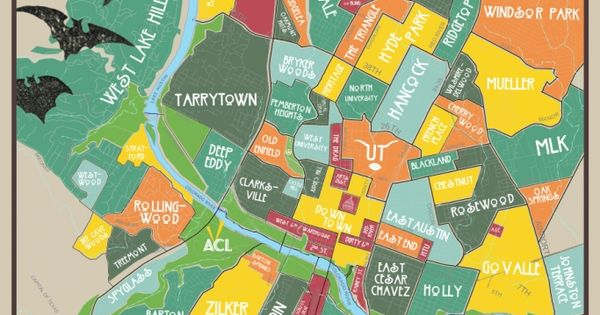
\includegraphics{austin.jpg} }
  			\setlength\fboxsep{0pt}
  			\setlength\fboxrule{0.5pt}
  		\end{figure}  \pause
  			
  		
  		Look up each house price?  \pause
  		
  		There are 360,000 houses in Austin --- is there a better way?
    \end{center}
    \end{frame}    
    
    
    
    \begin{frame}[label=lists]{Sample vs Population}
    	A faster approach: \pause
   		\begin{itemize}
   			\item Pick $n$ houses randomly (e.g. $n=100$) \pause
   			\item Take the average of the prices of these $n$ houses \pause
   			\item Hope that our estimate is close to the true mean price \pause
   		\end{itemize}
   		
   		% Emphasize that the sample should be selected randomly to avoid any biases.
   		
		Just like making polls to predict election results!
		
    \end{frame}    



    \begin{frame}[label=lists]{Sample vs Population}
    	
		
		%\begin{itemize}
   		%	\item Population $\leftarrow$ all houses in Austin
		%	\item Sample $\leftarrow$  $n$ houses you picked
	%		\item Population mean $\leftarrow$ Average house price in Austin
	%		\item Sample mean $\leftarrow$ Your estimate 			
   		%\end{itemize}
   		
		\begin{table}[!b]
        {\carlitoTLF % Use monospaced lining figures
        \begin{tabularx}{\textwidth}{Xcc}
          \textbf{} & \textbf{Population} & \textbf{Sample} \\
          \toprule
          Members       		 & all houses  & houses you selected  \\
          Mean               & population mean ($\mu$)    & sample mean ($\hat\mu$) \\
          SD & population SD ($\sigma$)   & sample SD ($\hat\sigma$) \\
          \bottomrule
        \end{tabularx}}
        
      \end{table} \pause
      \quad \newline    		
   		
   		We will estimate a \alert{population parameter} (population mean) based on a \alert{sample statistic} (sample mean).
		
    	%We could also estimate other population parameters, such as variance using the sample variance.
		
    \end{frame}  
 

    \begin{frame}[label=lists]{Collecting a sample}
    
    \begin{columns}[onlytextwidth]
        \column{.45\textwidth}
        	\begin{itemize}
          \item Go to \url{zillow.com} and search for Austin, TX.
   				\item Click ``More Map.''
   				\item Select 15 houses (try to get houses from all over town in a representative way), noting their prices in an R script. 
   				\item Do not discard any price, use the first 15 you find.
			\end{itemize}
        
         
        \column{.5\textwidth} 
        	
        	\begin{figure} 
				\centering
				\scalebox{.35}{ 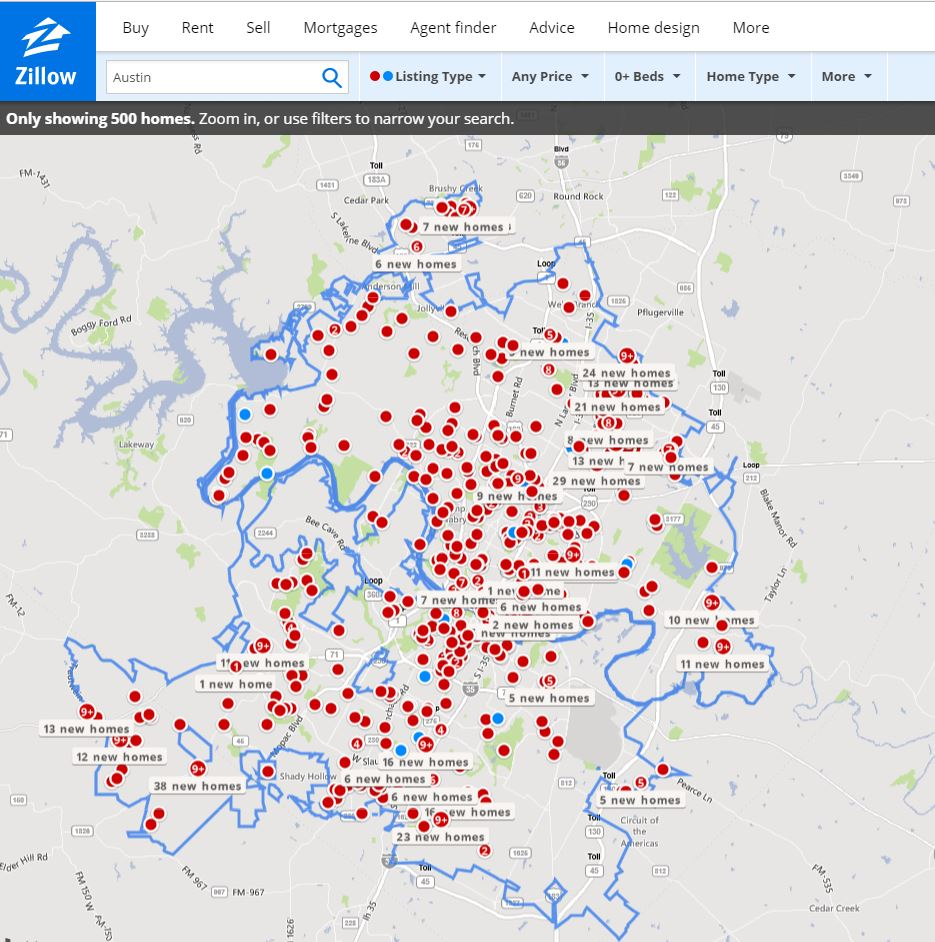
\includegraphics{zillow.jpg} }
				\setlength\fboxsep{0pt}
				\setlength\fboxrule{0.5pt} 
			\end{figure} 	
        	        
        \end{columns}
					
    \end{frame}  
    
    
    
    
    	\defverbatim[colored]\sampleZillow{
      \begin{lstlisting}[language=R,tabsize=2]
# Create a vector of house prices (you should have 15 prices)
sample_house_prices <- c(327000, 276000, 513000)
# Calculate sample statistics
sample_mean <- mean(sample_house_prices)
sample_variance <- var(sample_house_prices)
sample_standard_deviation <- sd(sample_house_prices)
# Sample mean of first 5 houses
sample_mean_5 <- mean(sample_house_prices[1:5])
    \end{lstlisting}}	
    
    \begin{frame}[label=lists]{Collecting a sample}
      \sampleZillow    
    \end{frame}


  %   \begin{frame}[label=lists]{Sampling Distribution} 
		% On Learning Catalytics, enter your results. \newline
		
		% And here is what they look like... % Use sample mean with 15 houses.
  %   \end{frame}



    \begin{frame}[label=lists]{Sampling Distribution}
    	%Everyone found a different sample mean, which one is correct?
    	%None. \newline %But they should be all clustered around the true mean (the average house price in Austin). \newline
    	
		Distribution of your answers  $\rightarrow$ \alert{Sampling distribution} \newline 
		    	
    	%Sample mean (your answers) itself has a distribution, separate from the house price distribution in Austin. This is called  \alert{sampling distribution}. \newline
    
    	
		\begin{table}[!b]
        {\carlitoTLF % Use monospaced lining figures
        \begin{tabularx}{\textwidth}{Xcc}
          \textbf{Statistic} & \textbf{Population} & \textbf{Sampling Distribution} \\
          \toprule
          Mean       		& $\mu$  & $\mu$  \\
          %Variance          & $\sigma^2$     & $\sigma^2/n$  \\
          Standard Deviation          & $\sigma$     & $\sigma/\sqrt{n}$ \\
          \bottomrule
        \end{tabularx}}
        
      \end{table}    	
      \quad \newline
      %What would you expect if you had 10\,000 houses in your survey?
    	
    	
		
    \end{frame}
    
       

	
	
	\begin{frame}[label=lists]{Sampling Distribution}
		\begin{figure} 
				\centering
				\scalebox{.5}{ 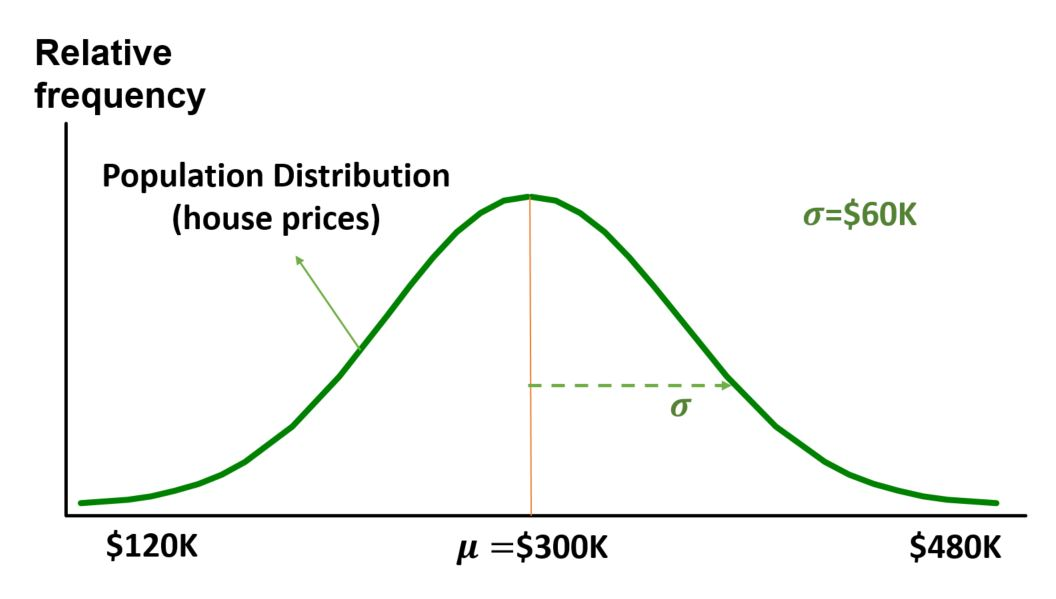
\includegraphics{sampling_1.jpg} }
				\setlength\fboxsep{0pt}
				\setlength\fboxrule{0.5pt} 
			\end{figure} 	
	\end{frame}	
	
	
		\begin{frame}[label=lists]{Sampling Distribution}
		\begin{figure} 
				\centering
				\scalebox{.5}{ 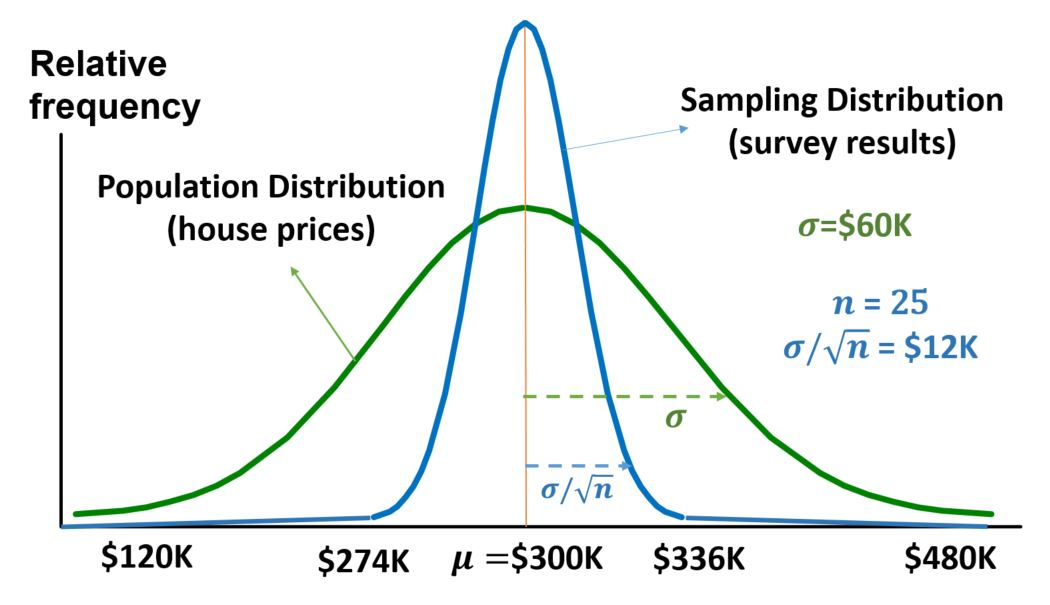
\includegraphics{sampling_2.jpg} }
				\setlength\fboxsep{0pt}
				\setlength\fboxrule{0.5pt} 
			\end{figure} 	
	\end{frame}	
    
    
    
    \begin{frame}[label=lists]{Sampling Distribution}
    
    Assume $\mu=\$300K$, $\sigma=\$60K$. \newline
    
   	\begin{table}[!b]
        {\carlitoTLF % Use monospaced lining figures
        \begin{tabularx}{\textwidth}{Xccc}
          \textbf{} &  $n$ & $\sigma/\sqrt{n}$  & $\pm 3\,\text{SD}$ range (99.7\%) \\
          \toprule
          Survey 1     & 25   &  \$12K	&\$264K ............. \$336K   \\
          Survey 2     & 100  &  \$6K	&\$282K ....... \$318K   \\
		  Survey 3     & 3600 &  \$1K	&\$297K ... \$303K   \\
          \bottomrule
        \end{tabularx}}	
	\end{table}   
    
    \end{frame}
    
    
	\begin{frame}[label=lists]{Sampling Distribution}
		Let's compare sample mean of 5 houses vs 15 houses. \newline
		
		What do you expect to see?
	\end{frame}
	

    
    
    \begin{frame}[label=lists]{$t$ Distribution}
    
    	We often do not know population variance and use sample variance instead. \newline
    	
    	
		In that case, the sample mean will have a \alert{$t$ distribution}.
	\end{frame}	
    
    
    
    \begin{frame}[label=lists]{Hypothesis Testing}
    Hypothesis: Average house price in Austin is \$1M. \pause
    
    Your survey on 25 houses: Average house price is \$$305K$. \newline \pause
    
    \begin{itemize}
      \item Would you reject the hypothesis? Why? \pause
      \item Is it possible that, out of bad luck, you picked the cheapest houses? \pause
      \item Would you be more comfortable with your conclusion if you had 1000 houses in your survey? \pause
      \item When should you reject the hypothesis? When not?
   \end{itemize}


	\end{frame}
	
	
	\begin{frame}[label=lists]{$p$-values}
		Your sample mean: $\hat\mu=\$305K$  \pause
	
    \begin{itemize}[<+->]
		  \item $H_0: \mu=\$1M$	(null hypothesis)
		  \item $H_1: \mu<\$1M$	(alternative hypothesis)
    \end{itemize}
		
		The \alert{$p$-value} is ``the probability of observing such an extreme ($\leq \$305K$) sample statistic if in fact the null hypothesis is true.'' \pause
		
		\begin{itemize}
		\item If $p < \alpha$, reject the null hypothesis \pause
		\item If $p \geq \alpha$, do not reject the null hypothesis \pause
		
		\end{itemize}		
		
		
		$\alpha$ is usually chosen as $0.05$ \underline{prior to sampling}.		
		
		% Ask how n would affect p value
		% Emphasize that the interpretation of p value is always the same.

	\end{frame}

  \begin{frame}
    \fullpagepicture{in-a-world}
  \end{frame}
	
	
	\begin{frame}[label=lists]{Let's assume we are in a world where $H_0$ is true...}
    \pause
		\begin{figure} 
				\centering
				\scalebox{.4}{ 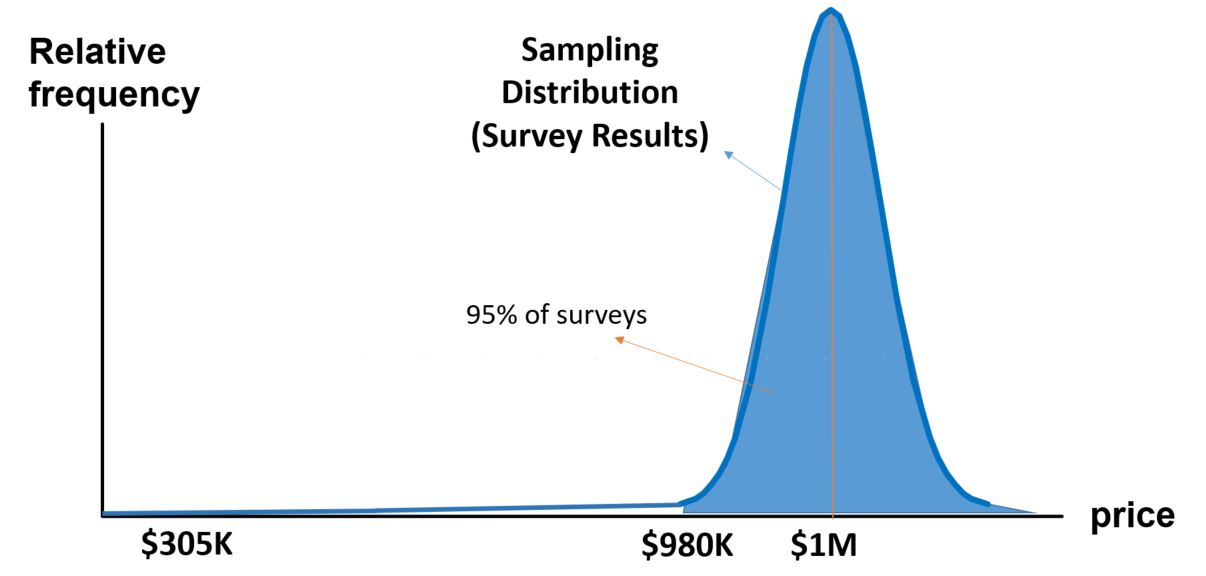
\includegraphics{pval2.jpg} }
				\setlength\fboxsep{0pt}
				\setlength\fboxrule{0.2pt} 
		\end{figure}
    \pause

    \begin{center}
      What is the probability of a sample where $\hat\mu\leq\$305K$? \pause
  		
      This is $p$, the area to the left of $\$305K$. $p<10^{-100}$!  \pause
		
		  Since $p<\alpha=0.05$, reject the null hypothesis!
    \end{center}
	\end{frame}
	
	
	% \begin{frame}[label=lists]{P-Value}
			
	% 		Learning Catalytics... \newline \pause
			
	% 		Your sample mean = \$305K. \newline \pause
			
	% 		$H_0$: Average house price is \$390K.
			
	% 		Would you reject the hypothesis? 
			
	% 		P-value = 0.01, $\alpha$=0.05 \newline \pause 
			
	% 		$H_0$: Average house price is \$320K.
			
	% 		Would you reject the hypothesis? 
			
	% 		P-value = 0.34, $\alpha$=0.01 \pause 
			
		
	% \end{frame}

	

	
	\begin{frame}[label=lists]{Confidence Intervals}
    \begin{center}
		The sample mean is probably not exactly equal to the population mean, but it's almost certainly ``close.'' \pause

    \bigskip
				
		A \alert{confidence interval} is a range that includes the population mean with a certain level of ``confidence.'' \pause
    \end{center}
  \end{frame}

  \begin{frame}{Confidence Intervals}
		Each sample will have a different 95\% confidence interval, and 95\% of such intervals will contain the population mean:

		\begin{figure} 
				\centering
				\scalebox{.6}{ 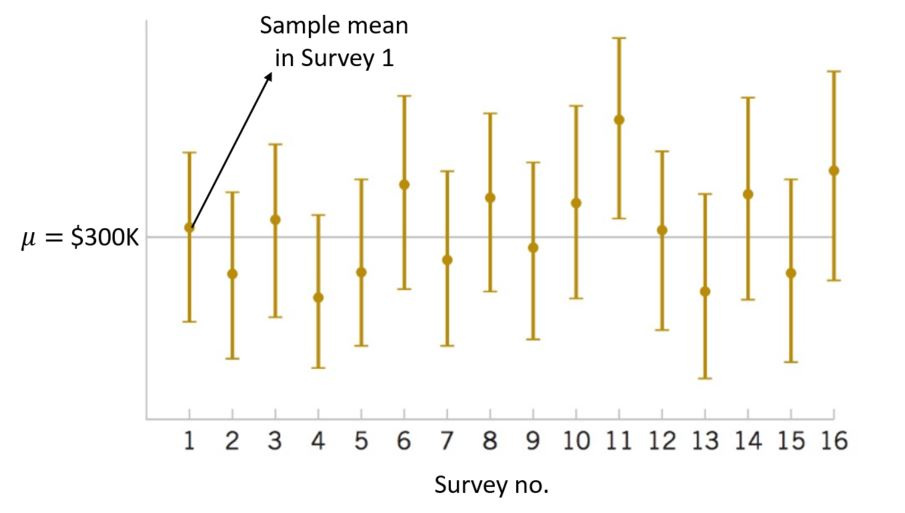
\includegraphics{confint.jpg} }
				\setlength\fboxsep{0pt}
				\setlength\fboxrule{0.2pt} 
		\end{figure} 	
		
	\end{frame}
	
	
    	\defverbatim[colored]\confInt{
      \begin{lstlisting}[language=R,tabsize=2]
# Calculate 95% confidence interval (default)
avg_price_ci_95 <- t.test(sample_house_prices, conf.level=0.95)
# Calculate 99% confidence interval
avg_price_ci_99 <- t.test(sample_house_prices, conf.level=0.99)
    \end{lstlisting}}	
    
    \begin{frame}[label=lists]{Confidence Interval}
      \confInt
    \end{frame}
	

\end{darkframes}
  
  
  

\end{document}

